\documentclass{article}

% if you need to pass options to natbib, use, e.g.:
% \PassOptionsToPackage{numbers, compress}{natbib}
% before loading nips_2016
%
% to avoid loading the natbib package, add option nonatbib:
%\usepackage[nonatbib]{report}

% to compile a camera-ready version, add the [final] option, e.g.:
\usepackage[square,sort,comma,numbers]{natbib}
\usepackage[final]{report}

\usepackage[utf8]{inputenc} % allow utf-8 input
\usepackage[T1]{fontenc}    % use 8-bit T1 fonts
\usepackage{hyperref}       % hyperlinks
\usepackage{url}            % simple URL typesetting
\usepackage{booktabs}       % professional-quality tables
\usepackage{amsfonts}       % blackboard math symbols
\usepackage{nicefrac}       % compact symbols for 1/2, etc.
\usepackage{microtype}      % microtypography
\usepackage{enumitem}
\usepackage{graphicx}

\title{CMP 719 - Computer Vision Assignment 1}

% The \author macro works with any number of authors. There are two
% commands used to separate the names and addresses of multiple
% authors: \And and \AND.
%
% Using \And between authors leaves it to LaTeX to determine where to
% break the lines. Using \AND forces a line break at that point. So,
% if LaTeX puts 3 of 4 authors names on the first line, and the last
% on the second line, try using \AND instead of \And before the third
% author name.

\author{
  Tayfun Ateş \\
  \texttt{n17230653@cs.hacettepe.edu.tr} \\
}

\begin{document}

\maketitle


\begin{abstract}

This document contains model details and experimental results conducted for the first assigment
of CMP719 course of the Department of Computer Engineering in Hacettepe University.

\end{abstract}

\section{Introduction}

 The deliverables of this homework is provided as a solution of a room classification problem with 15 classes. The classes tried to be learnt are fastfood restaurant, children room, bathroom, closet, tv studio, computer room, clothingstore, gym, auditorium, classroom, bar, garage, dining room, florist, bakery. Report contains three sections which are preparing data, training a classifier from scratch and transfer learning in convolutional neural networks. For the first two sections, a basic deep learning model, whose details are given in section 2, is selected. Experiments are conducted on top of this model and the model is updated if experiments result in an accuracy increase on the validation set incrementally. For the last section, instead of using a model created from scratch, we use Resnet18 model \cite{he2016deep} pre-trained with ImageNet dataset  \cite{russakovsky2015imagenet}. By the help of a famous model, we investigate effects of transfer learning. 
 
 During all experiments and tuning process, only validation test is used to update the best model. After reaching the best model for the validation set, accuracy result is given using test set. Using any data from test set during tuning parameters is considered as cheating and we also avoid doing that.

\section{Preparing Data}

As the dataset, we use MIT's indoor scene recognition dataset \cite{quattoni2009recognizing} which contains 67 indoor scene classes originally. We use only 15 of these classes to train our classifier. These 15 classes contain 2954 images in total. However, only a subset of those images is used for training and testing the model. Nearly 80 images for each category are selected for training and nearly 20 images for each category are selected for testing purposes summing 1229 train and 271 test images in total. Train set is also splitted so that 983 of the images are left to train set and 246 images are left to validation set. A random seed of 42 is used for splitting the train set. Splitting process is also stratified so that all classes are equally divided in the train and validation sets.

Dataloader for our data is implemented in dataset.py file. Transformations for the dataloaders are stated in config.py. There are basic transformations other than data augmentation which will be further investigated. Some of these basic transtionformations are scaling, resizing and normalizing. All images are converted to scale 0 and  1 and resized to a square size of 224. While finetuning the model pre-trained on ImageNet, the images are normalized with a mean of 0.485, 0.456, 0.406 and standard deviation of 0.229, 0.224, 0.225 for R, G and B channels in order to make our dataset's distribution similar to that of ImageNet.

We use a batch size of 32 which is chosen by considering our memory resources. For each batch in the train set,  we shuffle our dataset using our dataloader to provide stochasticity. We use a batch size of 1 for test and validation sets and we do not shuffle them.

In the next section, we will define our base model and explore whether different techniques are able to improve it or not. In this section, we explore whether augmenting data increases our accuracy on validation set or not. We train our base model twice with and without data augmentation. If the model trained with data augmentation achieves higher accuracy scores, we will keep data augmentation for the next experiments, if it does not we will not apply any data augmentation for the next experiments.

The data augmentation transformations that we have experimented are random resized crop of size 128 by 128 and random horizontal flip. We have trained these two models as mentioned in the next section. For this and the next experiments, accuracy is defined as the correctly identified samples to the total number of samples. Without any augmentation, our base model has a best validation accuracy of 0.35 among different epochs. With the data augmentation mentioned above, this best accuracy is increased to 0.43. Therefore, for the next experiments, we will train our model with data augmentation.

\section{Training a Classifier from Scratch}

In this section, we define our base model and experiments conducted on top of it. Our base model contains the following layers:

  \begin{enumerate}
    \item A convolutional layer with input channel size of 3, stride size of 1 and containing 32 filters of size 3 by 3
    \item A ReLU layer
    \item A convolutional layer with input channel size of 32, stride size of 1 and containing 64 filters of size 3 by 3
    \item A ReLU layer
    \item A max pool layer with a size of 2 by 2
    \item A convolutional layer with input channel size of 64, stride size of 1 and containing 128 filters of size 3 by 3.
    \item A ReLU layer
    \item A max pool layer with a size of 2 by 2
    \item A fully connected layer to obtain feature vectors of size 512
    \item A fully connected layer to obtain class probabilities
  \end{enumerate}%
  
None of the layers above contained padding to input tensors provided. We have used a relatively small network since our dataset is also small. Other types of layers such as dropout and batch normalization will further be investigated on top of our base network whether they help us or not.

As you can see, we use two fully connected layers from which the first one used to convert tensor representation to a vector representation of size 512 as in Resnet18. By using a vector of same size with Resnet18, it will be much meaningful to compare two networks for their power of image representation.

As also can be seen, ReLU layers are used as activation functions. There are several advantages of using ReLUs as activation functions. One reason is that ReLU is very robust against gradient vanishig problem. However, this has less importance since our base network is not deep a lot. Other and more important reason for using ReLU is that it provides constant gradient value resulting faster training when compared for example to sigmoid. Since this is a homework and it is required to see the results quickly, it is a natural choice using ReLU activations.

A natural choice when dealing with multi-class classification problem is to use cross entropy loss after a softmax activation. We also use this loss function.

All of the models are trained with Adam optimizer. We use Adam because of its convergence speed and robustness to different values of hyperparameters. Learning rate is tuned by observing loss values among different batches for our dataset using both our model and Resnet18. For the experiments deciding whether data augmentation is helpful or not, we use a learning rate of 0.00025 and a weight decay of 0.0005. However, when experimenting batch normalization and dropout, learning rete is updated in order to achieve faster convergence.

First experiment that we have conducted on top of our base model with data augmentation is to check whether using batch normalization layers after each convolution layer increases our validation accuracy or not. Batch normalization is a technique providing tensors to next layers with zero mean and unit variance. Since batch normalization layers add some noise into the network, they can be seen in a way as regulizers. We have trained our model 150 epoch with a learning rate of 0.00025 and obtained a validation accuracy of 0.53 in the latest epochs. Besides showing that batch normalization layers can increase the validation accuracy of our model, this experiment showed that we need to train more with higher number of epochs and/or learning rate in order not to underfit our model.

The next and the last experiment that we have conducted on top our model with batch normalization layers is to check if using dropout in the first fully connected layer to drop some features increases our validation accuracy or not. We have experimented with a dropout probability of 0.25. We have first increased number of epochs to 1000 by fixing the learning rate to 0.00025 and obtained  a best validation accuracy of 0.60. Although this experiment tooks a little bit long, further experiments on learning rate and the number of epochs have reached similar best validation accuracy at maximum. Furthermore, increasing learning rate much has resulted in instable traning where validation scores drop significantly.

We have observed that data augmentation, batch normalization and dropout, all together, increase our best validation accuracy score from 0.35 to 0.60. You can find in Figure \ref{fig:myTrainingProcess} our best model's training behaviour for both training loss and validation accuracy using a batch size of 32, learning rate of 0.00025 and total number of epochs 1000. Loss is calculated for a batch and averaged for an epoch, validation accuracy is calculated after 5 epochs. This is why loss plot is more dense compared to validation accuracy plot. We plotted validation accuracy instead of validation loss without losing any important information. Accuracy and loss of validation have inverse relationship. After 1000 epoch of training, both training loss and validation accuracy start to converge. To avoid overfitting, we apply early stopping by saving model outputs of the each epoch for which validation testing runs. As can be seen from blue plot, we obtained our best model from the output of 845. epoch where the validation accuracy is the highest.

\begin{figure}
  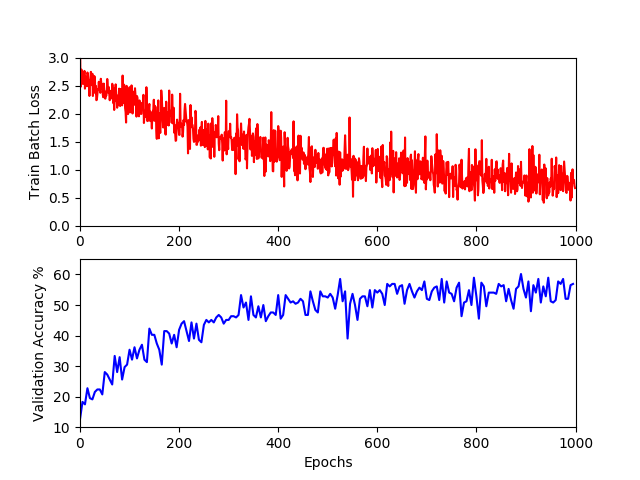
\includegraphics[width=\linewidth]{myTrainingProcess.png}
  \caption{Training loss and validation accuracy for epochs}
  \label{fig:myTrainingProcess}
\end{figure}

TODO
Test best model on best model

In conclusion, we have investigated creating and training a model for a room classification problem from scratch. This model could also be improved with more data augmentation and exploring dropout not only with a probability of 0.25 but also with higher values. The performance of this model could also be improved by introducing much data. Moreover, as can also be seen in the next section, this model first could be trained on a larger dataset (possibly ImageNet) for a different problem and then finetuned for room classification problem. This transfer learning process could also improve the performance of our naive model.

\section{Transfer Learning in Convolutional Neural Networks}

Details about finetuning go here 


\section{Conclusions}
 
{\small
\bibliographystyle{ieee}
\bibliography{report}
}


\end{document}
